\documentclass[xcolor=table]{beamer}
%\def\infinity{\rotatebox{90}{8}}
\usetheme{Cranfield}
\usepackage{amsfonts}
\usepackage[utf8]{inputenc}
\usepackage{float}
\usepackage{multimedia}
\setbeamertemplate{navigation symbols}{}
\usepackage{times}
\usepackage[T1]{fontenc}
\usepackage{multirow}

\title{Multiphase implementation on a parallel 2D/3D Lattice Boltzmann solver
	using GPGPUs}
\subtitle{Technical Presentation}
\author{José Oliveira}
\institute{Cranfield University\\ School of Aerospace, Transport and Manufacturing}
\date{July 2017}


\begin{document}
	\begin{frame}
		\titlepage
	\end{frame}
	
	\begin{frame}
		\frametitle{Index}
		\begin{enumerate}
			\item Introduction
			\item Multiphase Lattice Boltzmann Methods
			\item Result
			\item Future work
		\end{enumerate}
	\end{frame}
	
	\begin{frame}
		\frametitle{Lattice Boltzmann Method}
		\framesubtitle{Applications}
		\begin{block}{What is the Lattice Boltzmann Method?}
		LBM is a fluid flow simulation method capable of solving CFD problems.
		\end{block}
		\begin{itemize}
			\item Incompressible and isothermal flows
			\item Mesoscopic approach
			\item Model evolution of time
			\item Commonly used in automotive industry
			\item Great candidate for parallel programming
		\end{itemize}
	

	\end{frame}
	\begin{frame}
		\frametitle{Multiphase flow in Lattice Boltzmann}
		\begin{columns}
			\column{0.5\textwidth}
		Multiphase can simulate flows in different states
		\begin{itemize}
			\item Solid / Liquid
			\item Liquid / Liquid
			\item Gas / Solid
			\item etc.
		\end{itemize}
		Used in
		\begin{itemize}
			\item Problems controlled by surface tension
			\item Oil industry
			\item Bubble dynamics
			\item Fluid management in space
		\end{itemize}

		\column{0.5\textwidth}
		\begin{figure}
			\centering
			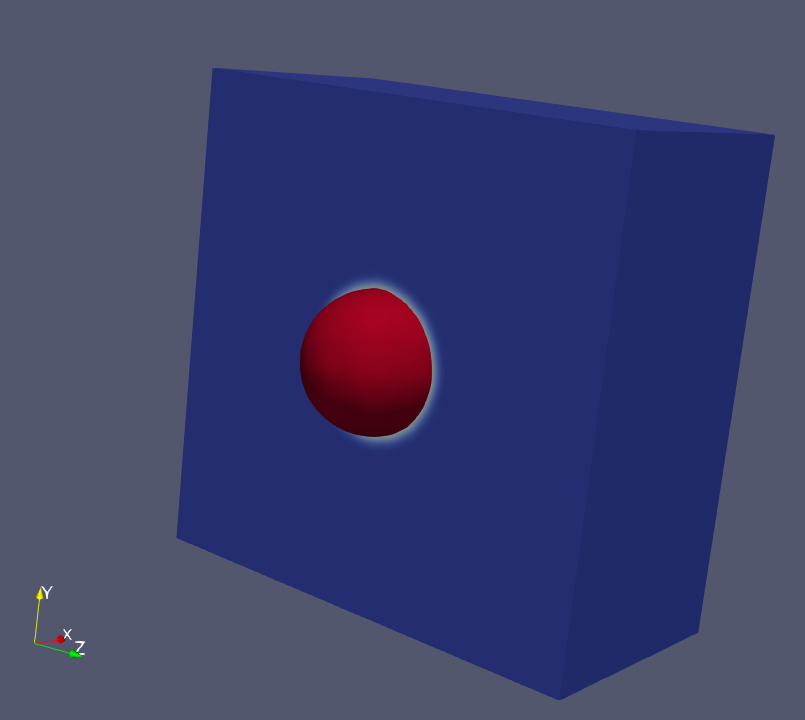
\includegraphics[scale=0.2]{Resources/3DCG.png}
		\end{figure}
		\end{columns}
	\end{frame}
	\begin{frame}
		\frametitle{High Performance Computing}
				\begin{figure}
					\centering
					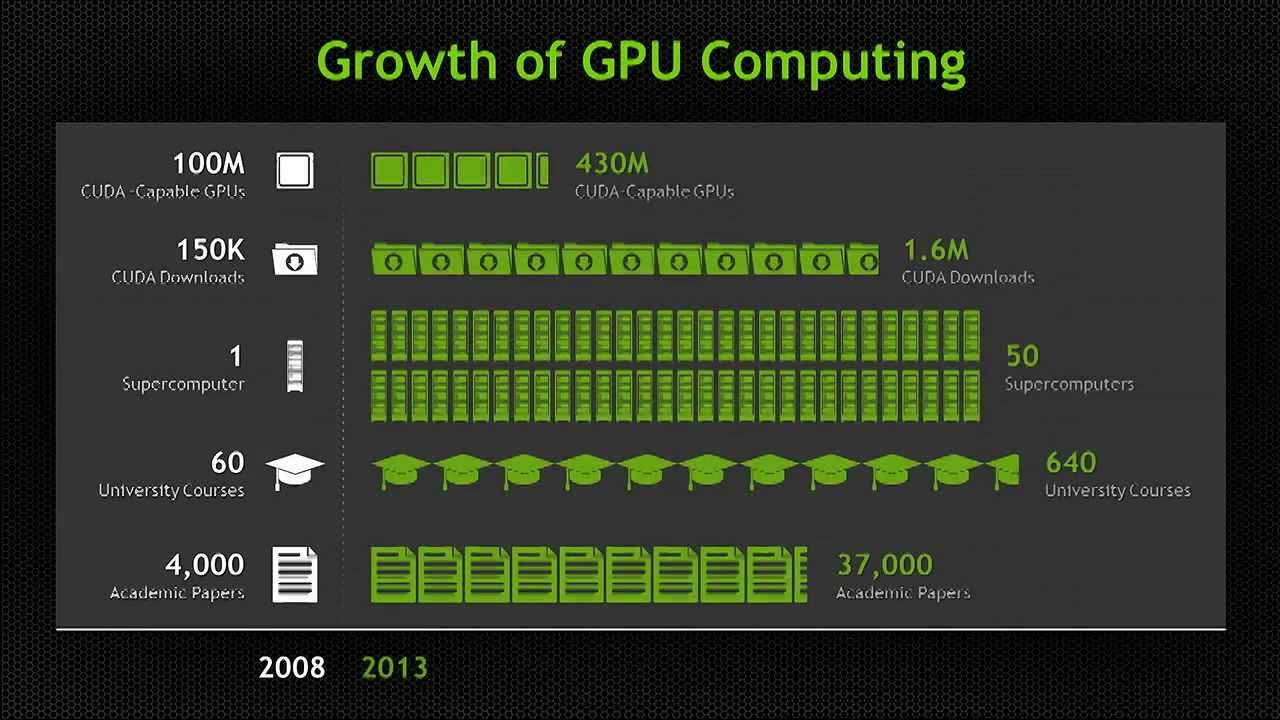
\includegraphics[scale=0.25]{Resources/gpuEvo.jpg}
				\end{figure}
	\end{frame}
	\begin{frame}
		\frametitle{Cuda Programming}
		\begin{columns}
		\column{0.5\textwidth}
		Main differences from CPU programming
		\begin{itemize}
			\item Different memory structure (registers, shared, constant and global memory)
			\item Many concurrent threads
		\end{itemize}

		\column{0.5\textwidth}
		\centering
			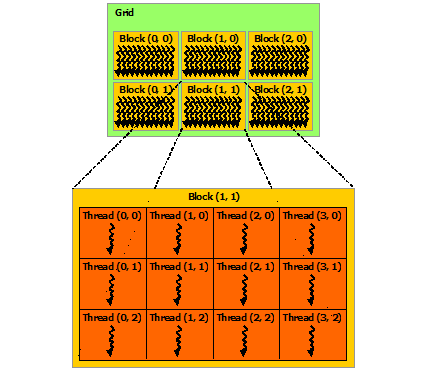
\includegraphics[scale=0.6]{Resources/grid-of-thread-blocks.png}
	\end{columns}
	\end{frame}
	\begin{frame}
		\frametitle{Lattice Boltzmann Method}
		\framesubtitle{Basics}
		\begin{columns}
			\column{0.5\textwidth}
			Iterative method, analogous from 2D to 3D
			\begin{enumerate}
				\item Collision
				\item Streaming
				\item Boundary conditions
				\item Macro-variable update
				\item Residuals
			\end{enumerate}
			\column{0.5\textwidth}
			\centering
			\begin{figure}[t]
				\centering
			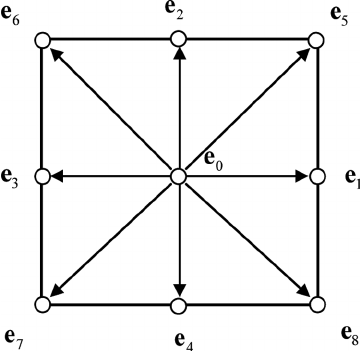
\includegraphics[scale=0.25]{Resources/d2q9.png}
			\end{figure}
			\begin{figure}[b]
				\centering
			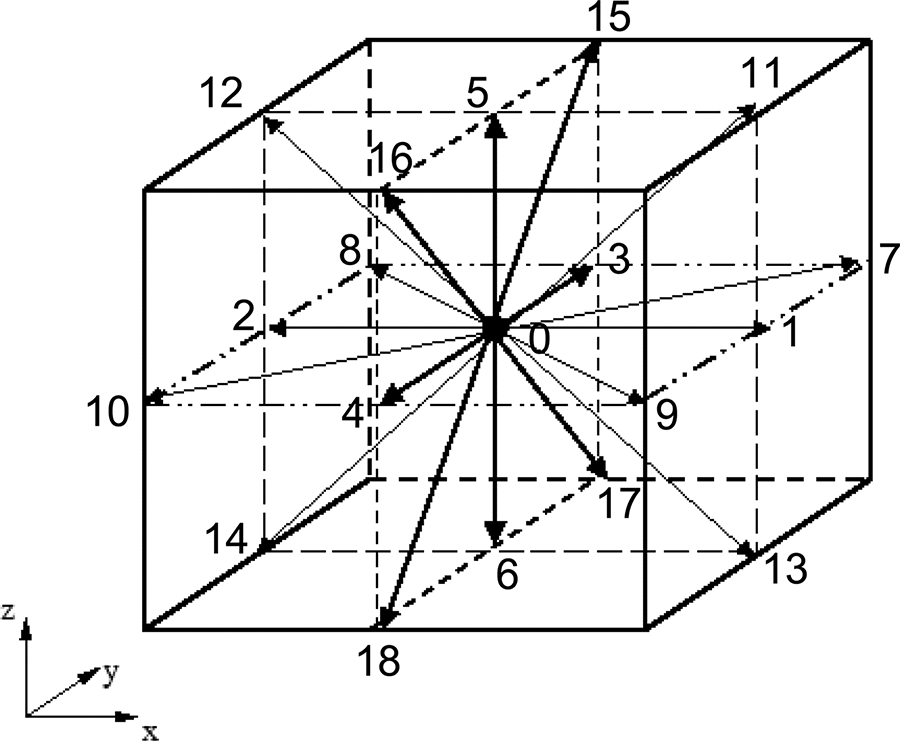
\includegraphics[scale=0.15]{Resources/d3q19.png}
		\end{figure}
		\end{columns}
	\end{frame}
	\begin{frame}
		\frametitle{Color Gradient Model}
		Simulates interaction between a red and blue fluid.
		\begin{itemize}
			\item Single phase collision
			\item Perturbation
			\item Recoloring
		\end{itemize}
		Plans for implementation:
		\begin{enumerate}
			\item 2D case
			\begin{itemize}
				\item Serial
				\item Validation
				\item Parallel
				\item Validation
			\end{itemize}
					\item 3D case
		\end{enumerate}
		
	\end{frame}
		\begin{frame}
		\begin{center}
			\Huge \textcolor{cranfieldblue}{Results}
		\end{center}
		\end{frame}
						\begin{frame}
							\frametitle{Previous solver}
							\framesubtitle{Runtimes}
							\begin{figure}
								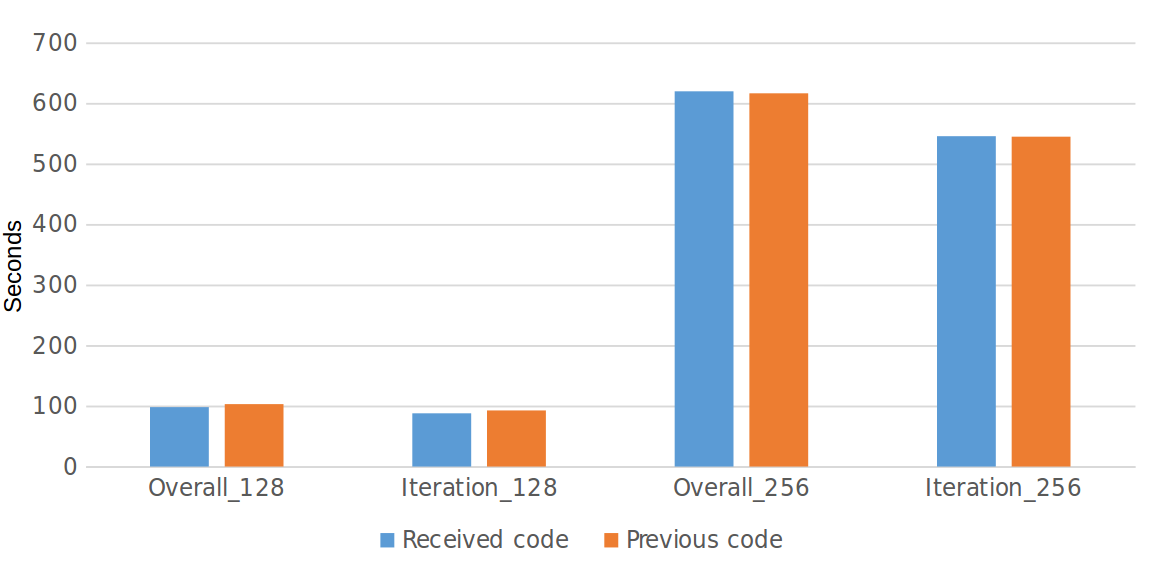
\includegraphics[scale=0.25]{Resources/compareTimes.png}
							\end{figure}
						\end{frame}
						\begin{frame}
							\frametitle{Previous solver}
							\framesubtitle{Validation}
							\begin{textblock*}{5cm}(-0.8cm,-2.5cm)
							\begin{figure}
								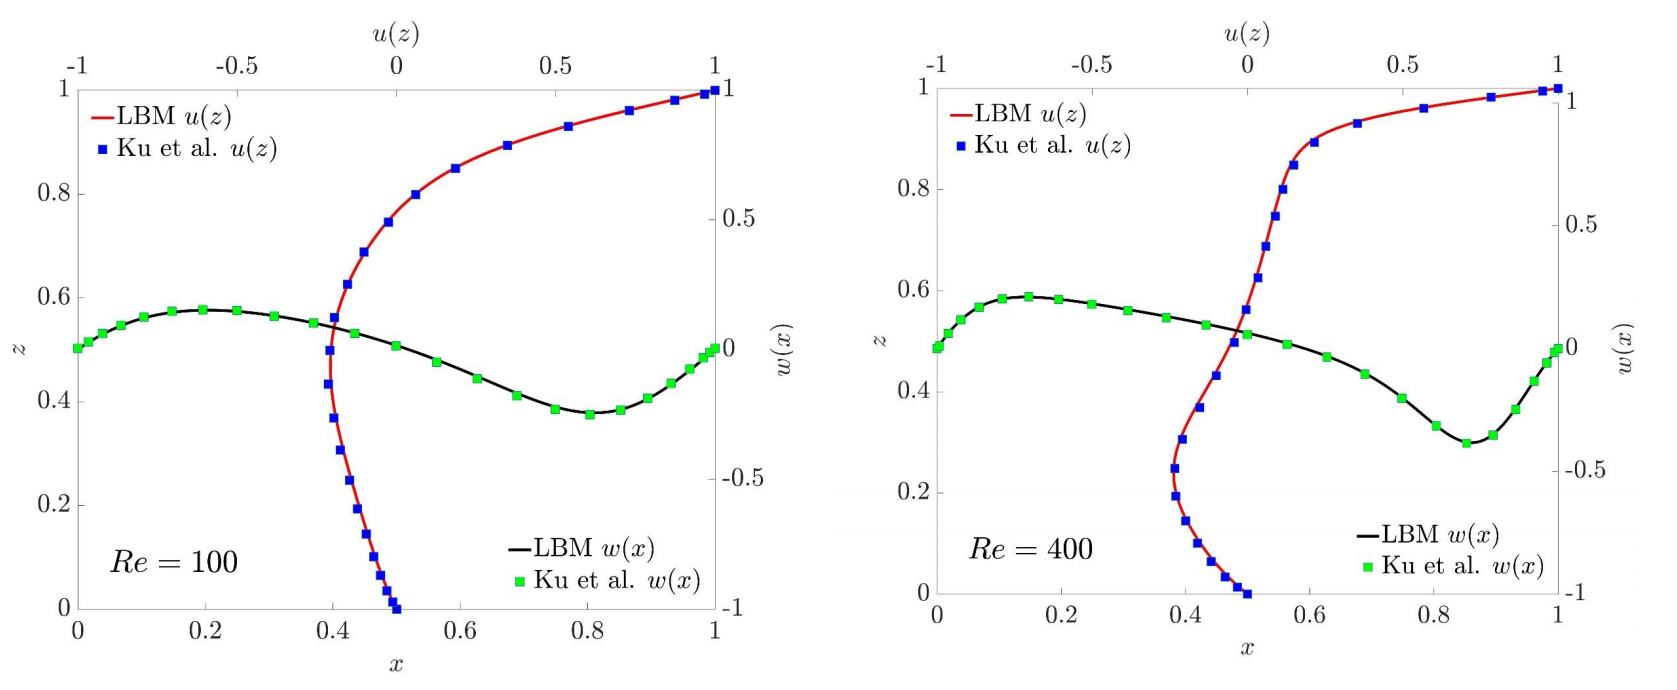
\includegraphics[scale=0.215]{Resources/prevValid.png}
							\end{figure}
							\end{textblock*}
						\end{frame}
		\begin{frame}
			\frametitle{Validation}
			\framesubtitle{Coalescence and oscilation}
			\begin{textblock*}{5cm}(0cm,-3.3cm)
				\movie[label=show3,scale=0.2,
				,autostart,loop] 
				{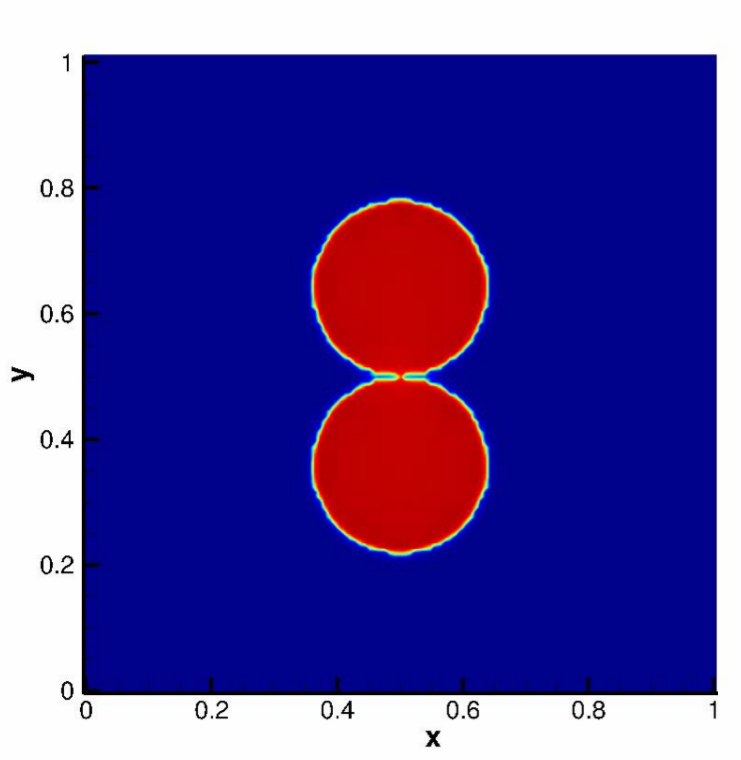
\includegraphics[scale=0.2]{Resources/coalescence.png}}{Resources/coalescence.mp4}
			
			\end{textblock*}
			\begin{textblock*}{5cm}(1cm,2cm)
			\begin{table}[]
				\centering
				\begin{tabular}{c|clll}
					$\gamma$ & Error (\%) &  &  &  \\ \cline{1-2}
					1      & 4.81       &  &  &  \\
					10     & 0.56       &  &  &  \\
					40     & 0.93       &  &  &  \\
					75     & 0.16       &  &  & 
				\end{tabular}
			\end{table}
			\end{textblock*}
			\begin{textblock*}{5cm}(5.4cm,-3.2cm)
					\movie[label=show3,scale=0.2,autostart
					,loop] 
					{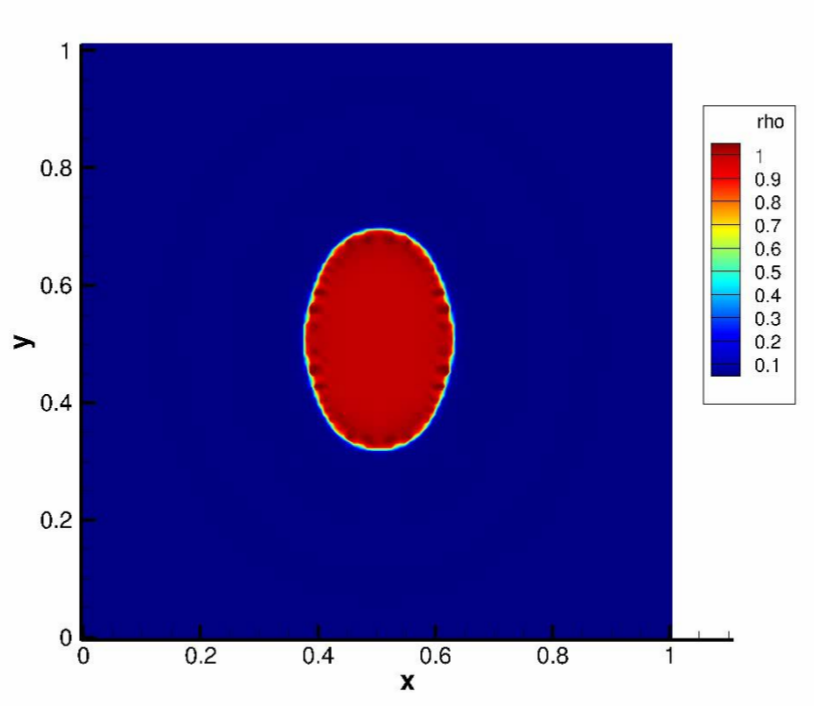
\includegraphics[scale=0.2]{Resources/oscil.png}}{Resources/oscilating.mp4}
			\end{textblock*}
				\begin{textblock*}{5cm}(5.3cm, 1.7cm)
					\begin{figure}
						\centering
						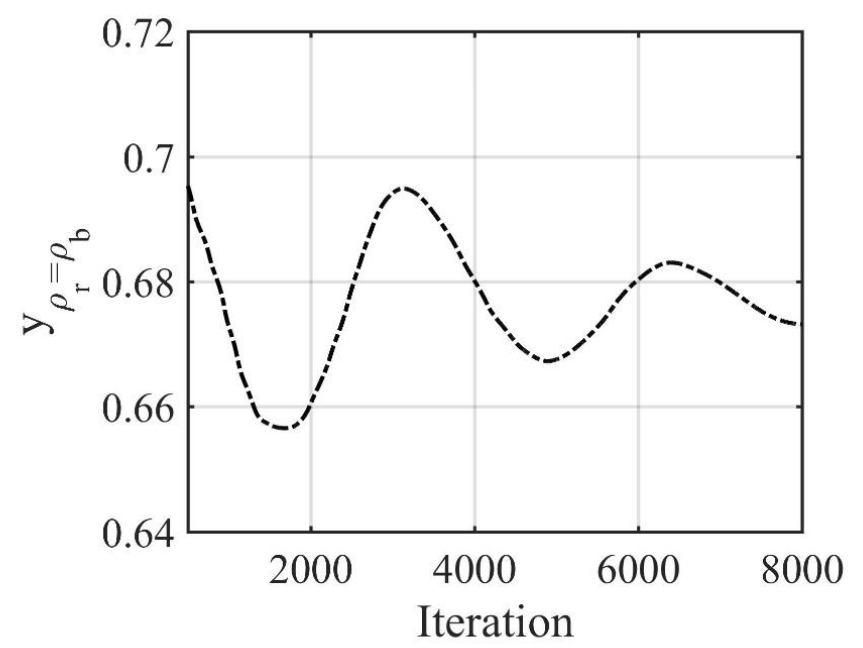
\includegraphics[scale=0.13]{Resources/oscilValid.png}
					\end{figure}
				\end{textblock*}
		\end{frame}
		\begin{frame}
			\frametitle{Validation}
			\framesubtitle{Couette flow}
			\begin{figure}
				\centering
				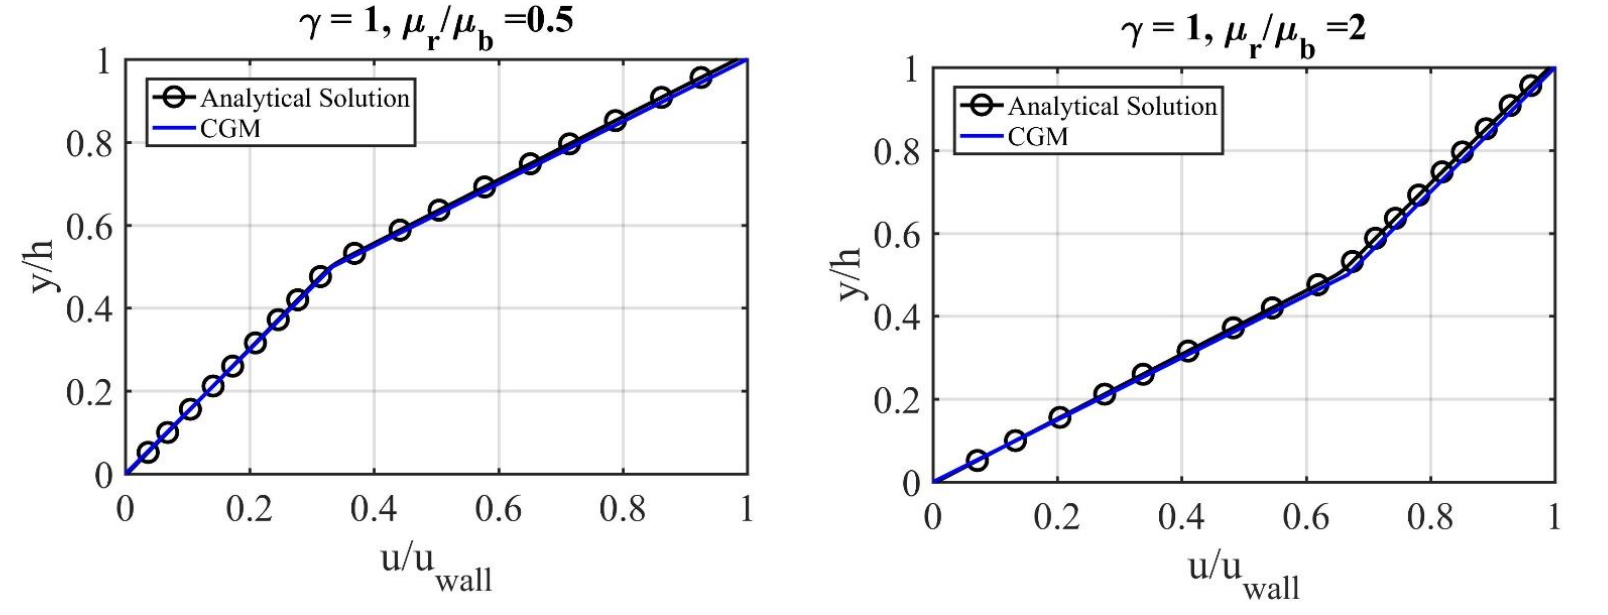
\includegraphics[scale=0.2]{Resources/couette.png}
			\end{figure}
			\small Validated by Antonio González, MSc CFD Thesis at Cranfield University
		\end{frame}
		\begin{frame}
			\frametitle{Memory usage}
	\small
	\begin{textblock*}{5cm}(-0.5cm,-0.7cm)
\begin{table}[]
	\centering
	\begin{tabular}{l|lll}
		\textbf{Type}    & \textbf{Nodes} & \textbf{Single precision (MB)}                     & \textbf{Double Precision (MB)}                     \\ \hline
		\textbf{2D\_128} & 16384                    & \cellcolor[HTML]{EFEFEF}21,8  & \cellcolor[HTML]{C0C0C0}33,6 \\
		\textbf{3D\_128} & 2097152                  & \cellcolor[HTML]{EFEFEF}1725                  & \cellcolor[HTML]{C0C0C0}2785                  \\
		\textbf{2D\_256} & 65536                    & \cellcolor[HTML]{EFEFEF}47,97 & \cellcolor[HTML]{C0C0C0}83,95 \\
		\textbf{3D\_256} & 16777216                 & \cellcolor[HTML]{EFEFEF}9637                  & \cellcolor[HTML]{C0C0C0}18091                
	\end{tabular}
\end{table}
\end{textblock*}
		\end{frame}
				\begin{frame}
					\frametitle{Performance}
						\begin{textblock*}{5cm}(0cm,-3.7cm)
							\begin{figure}
								\centering
								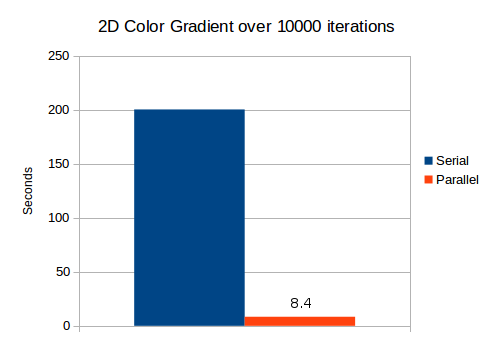
\includegraphics[scale=0.43]{Resources/2dperfor.png}
							\end{figure}
							\end{textblock*}
							\begin{textblock*}{5cm}(6cm,-3.7cm)
								\begin{figure}
									\centering
									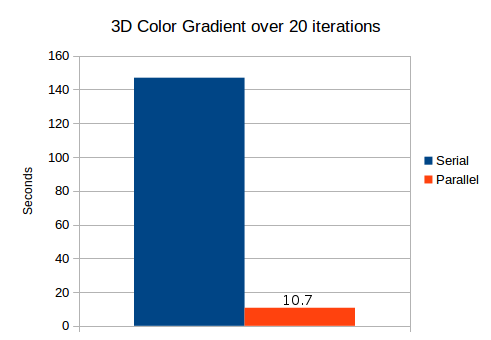
\includegraphics[scale=0.43]{Resources/3dperformance.png}
								\end{figure}
							\end{textblock*}
							\begin{textblock*}{5cm}(2.5cm,0.4cm)
								\begin{figure}
									\centering
									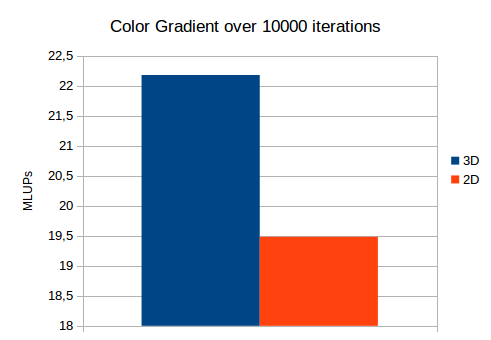
\includegraphics[scale=0.43]{Resources/performance.png}
								\end{figure}
							\end{textblock*}
							
				\end{frame}
				\begin{frame}
					\frametitle{Code profiling}
						\begin{figure}[l]
							\centering
							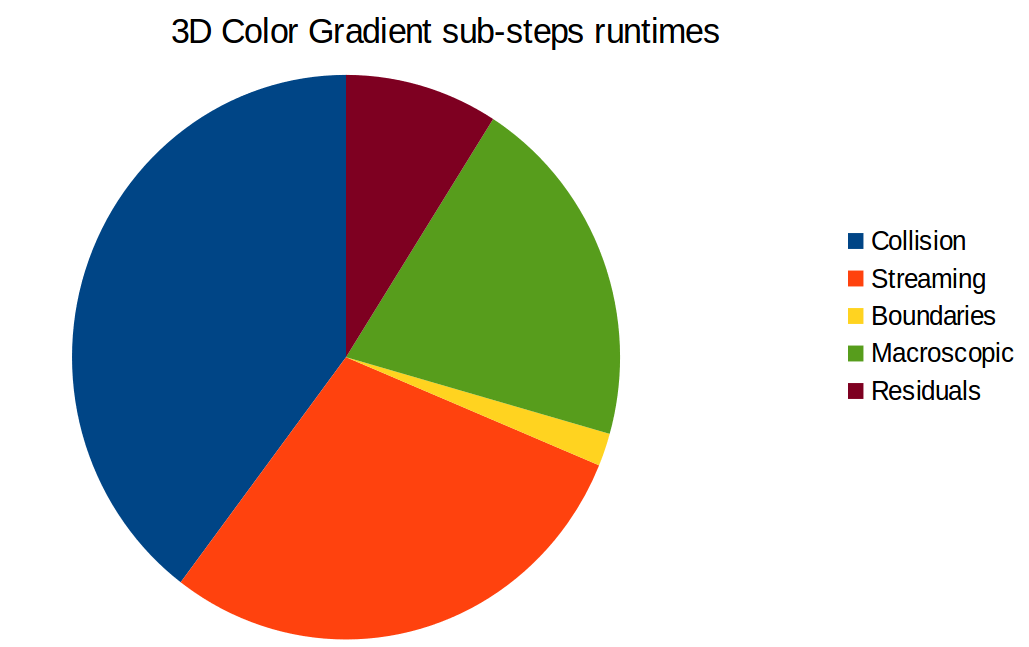
\includegraphics[scale=0.3]{Resources/3Dprofile.png}
						\end{figure}
				\end{frame}
				\begin{frame}
					\frametitle{Future work}
					\begin{itemize}
						\item Implement higher order Color Gradient
						\item Improve memory usage/performance
						\item Validate 3D solver
						\item Finish writing thesis
					\end{itemize}
				\begin{table}[]
					\centering
					\begin{tabular}{l|l|l|l|l|l}
						& \multicolumn{2}{c|}{July}                                                  & \multicolumn{3}{c|}{August}                                                    \\ \hline
						& 24 - 27                                         & 27 – 01                  & 2 – 8                    & 9 – 15                   & 15 – 18                  \\ \hline
						High Order CG & \cellcolor[HTML]{EFEFEF}                        &                          &                          &                          &                          \\ \hline
						3D Validation   & \cellcolor[HTML]{C0C0C0}{\color[HTML]{C0C0C0} } &                          &                          &                          &                          \\ \hline
						Optimisation    &                                                 & \cellcolor[HTML]{656565} & \cellcolor[HTML]{656565} &                          &                          \\ \hline
						Writing         &                                                 &                          & \cellcolor[HTML]{000000} & \cellcolor[HTML]{000000} & \cellcolor[HTML]{000000}
					\end{tabular}
				\end{table}
				\end{frame}
				\begin{frame}
					\centering
						\Huge \textcolor{cranfieldblue}{Thank you!}
				\end{frame}
\end{document}